
\chapter{Análise Bibliográfica sobre Segurança WEB via Token, por Allann Gois Hoffmann\label{chap:bibliometria:AllannH}}

\section{Sobre o tema}
Baseado no grande uso da internet nos dias de hoje para simples buscas, autenticações em sites ou compras online, a segurança dos dados que são trafegados são de imensa importância. Tendo como base esse conhecimento, essa pesquisa tem como objetivo realizar uma pesquisa bibliométrica em relação ao tipo de validação de segurança por meio de tokens para validar a permissão do usuário à informação.

\section{Ferramenta utilizada}
A analise do conjunto de dados foi feita na Linguagem R, por meio da ferramenta \textit{RStudio} e utilizando o pacote \textit{Bibliometrix} e a aplicação \textit{Biblioshiny}.

\section{Coleta de dados} 
A base de dados utilizada para busca foi a Web of Science (WOS), por meio do Periódicos da CAPES. Inicialmente foi utilizada todas as bases de dados, porém, devido ao grande numero de resultados a base foi alterada para somente a coleção principal da WOS e realizada no dia 07/02/2022.

\subsection{Querys utilizadas}
Na primeira busca foi utilizada todas as bases de dados para pesquisa:
```(web AND token) AND security```
Mas teve como retorno somente 864 resultados, e com isso a busca foi atualizada para:
```(token* AND (securit* OR WEB))````
Essa obteve 11,254 resultados, e para obter os melhores resultados a base utilizada foi alterada para a coleção principal, na qual teve 2678 resultados e que ao retirar todas as fontes que não são artigos sobrou 866, os quais foram utilizados na analise.

\section{Análise dos dados}

\subsection{Principais pontos}
O primeiro ponto a ser observado são os dados gerais sobre os artigos, e temos os principais como:
\begin{itemize}
\item Data de publicação: 1971:2022
\item Media de citações por documento: 12,75
\item Media de citação por ano de cada artigo: 1,55
\item Referencias: 27936 
\item Palavras-chave do autor: 2817
\item Documentos por autor: 0,334
\item Autor por documento: 2,99
\end{itemize}

\subsection{Número de artigos produzidos}

\begin{figure}
    \centering
    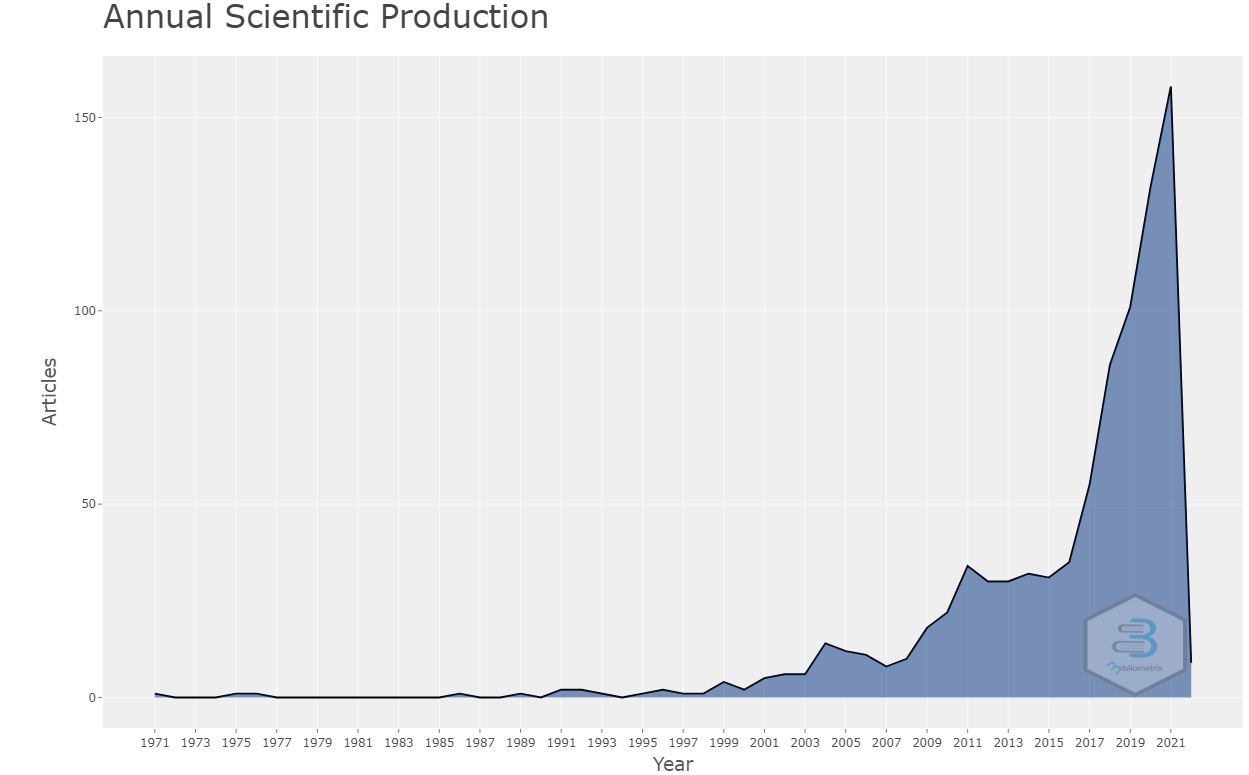
\includegraphics[width=1\textwidth]{experiments/AllannH/PesquisaBibliometrica/Imagens/TSW-AllannH-numero_producoes.png}
    \caption{Número de produção de artigos ao longo dos anos.}
    \label{fig:AllannH-num_prod}
\end{figure}

Na imagem \ref{fig:AllannH-num_prod} podemos ver que a partir de 1971 a segurança por meio de tokens de acesso já estava sendo estudados, e com o a entrada da internet a preocupação e o numero de pesquisas só aumentou, principalmente nos 5 últimos anos. 

\subsection{Media de citações por artigo}
Por meio da imagem podemos que o número de citações ao longo dos anos foi muito instável e com alguns picos como no ano de 2007, porém com uma tendencia de crescimento. Os anos com mais destaques são 2004 e 2013 com aproximadamente 4 citações e o ano de 2007 com a maior quantidade de citações com 6

\begin{figure}
    \centering
    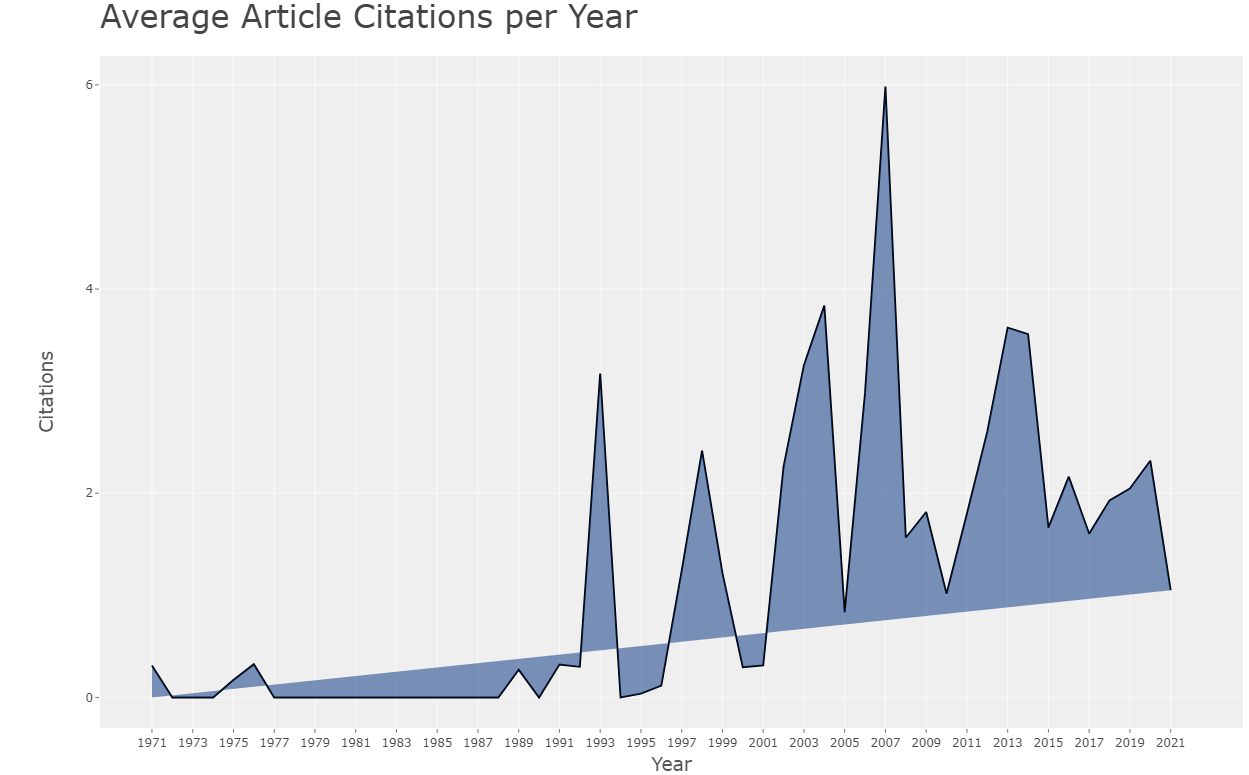
\includegraphics[width=1\textwidth]{experiments/AllannH/PesquisaBibliometrica/Imagens/TSW-AllannH-media_citacoes.png}
    \caption{Media de citações dos artigos durante os anos.}
    \label{fig:AllannH-media_citacoes}
\end{figure}

\subsection{Países mais relevantes}

Os países que mais se destacam são a China, Estados Unidos e Índia. Sendo que a China mostra um numero muito superior comparado com todos os outros países. Podemos comprovar observando a imagem \ref{fig:AllannH-paises_relevantes}

\begin{figure}
    \centering
    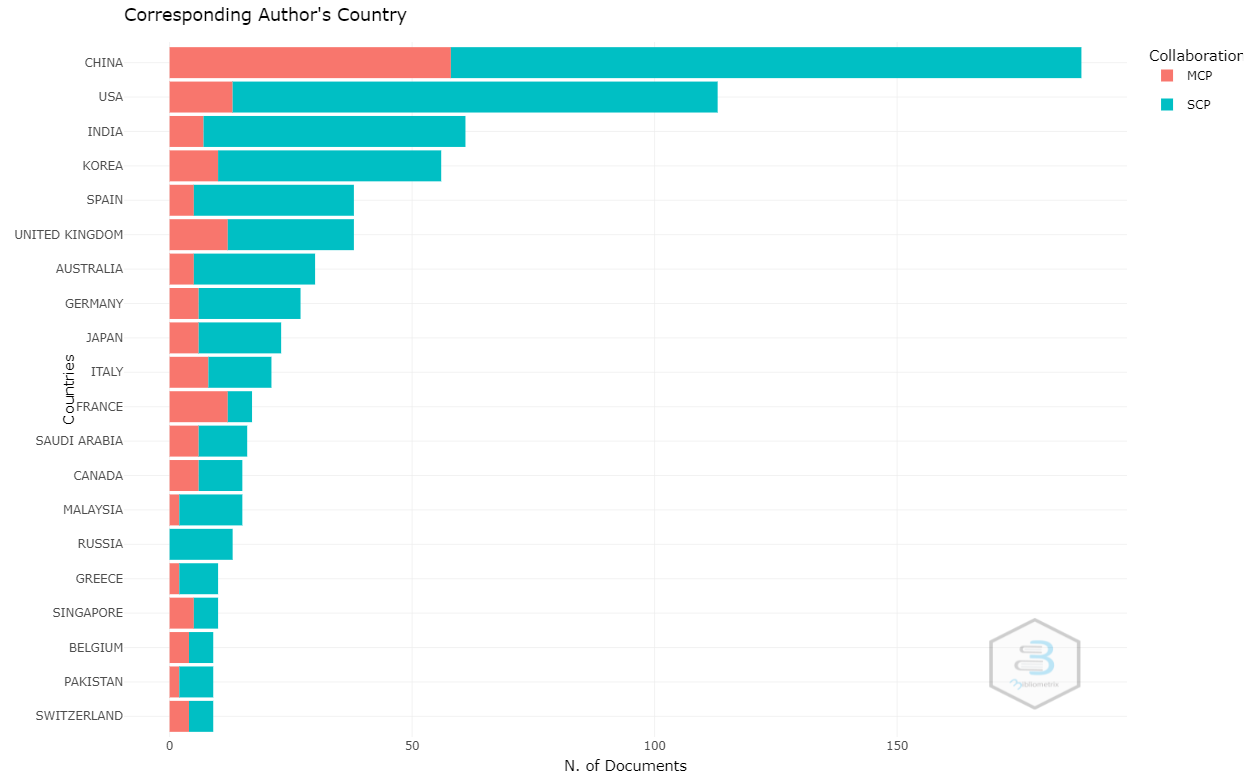
\includegraphics[width=1\textwidth]{experiments/AllannH/PesquisaBibliometrica/Imagens/TSW-AllannH-paises_relevantes.png}
    \caption{Países com o maior número de produção.}
    \label{fig:AllannH-paises_relevantes}
\end{figure}

\subsection{Universidades mais relevantes}

\begin{figure}
    \centering
    \caption{Universidade com o maior número de produção.}
    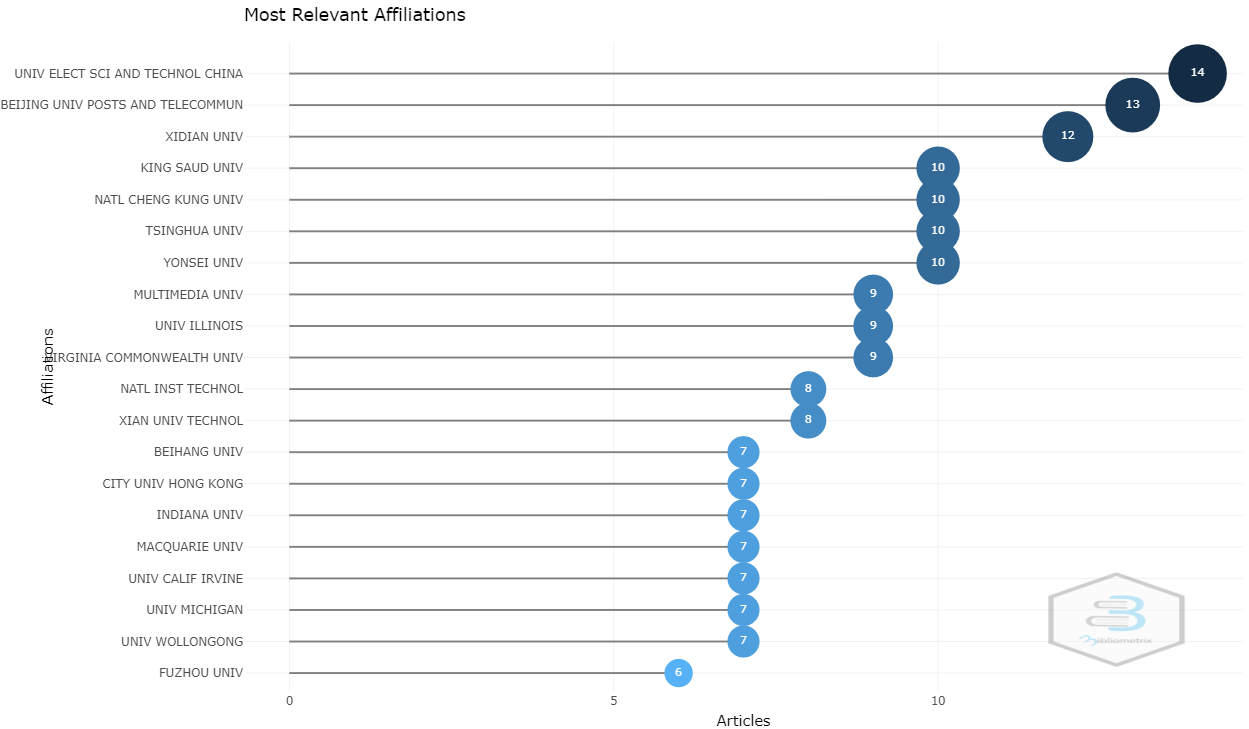
\includegraphics[width=1\textwidth]{experiments/AllannH/PesquisaBibliometrica/Imagens/TSW-AllannH-universidades_relevantes.png}
    \label{fig:AllannH-uni_relevantes}
\end{figure}
Observando a imagem \ref{fig:AllannH-paises_relevantes}, é de se imaginar o local das universidades mais relevantes. A imagem \ref{fig:AllannH-uni_relevantes} mostra que a maioria das universidades estão realmente localizadas na China.

\subsection{Principais fontes citadas}

\begin{figure}
    \centering
    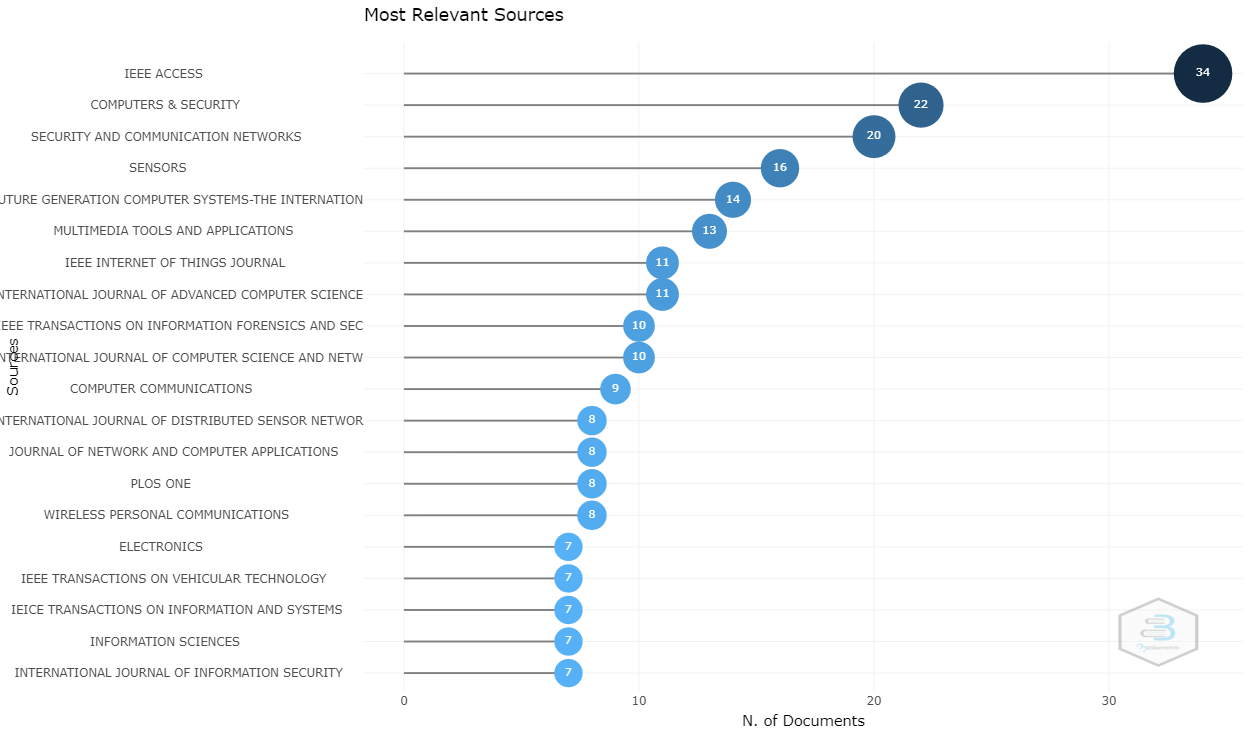
\includegraphics[width=1\textwidth]{experiments/AllannH/PesquisaBibliometrica/Imagens/TSW-AllannH-fontes_relevantes.png}
    \caption{Fontes mais relevantes no mercado.}
    \label{fig:AllannH-fontes_relevantes}
\end{figure}
Por meio da imagem \ref{fig:AllannH-fontes_relevantes} é possível ver o destaque de 3 fontes, sendo elas:
\begin{itemize}
\item IEEE ACCESS
\item COMPUTERS \& SECURITY
\item SECURITY AND COMMUNICATION NETWORKS
\end{itemize}
Analisando a diferença entre o número de publicações o destaque das 3 no mercado é nítido.

\subsection{Principais artigos citados}
Os artigos mais citados é possível serem analisados pela imagem \ref{fig:AllannH-artigos_citados}, e que os principais artigos tem um grande número de citações e dado o crescimento de produções somente nos últimos anos, é de se notar a data destes artigos citados.

\begin{figure}
    \centering
    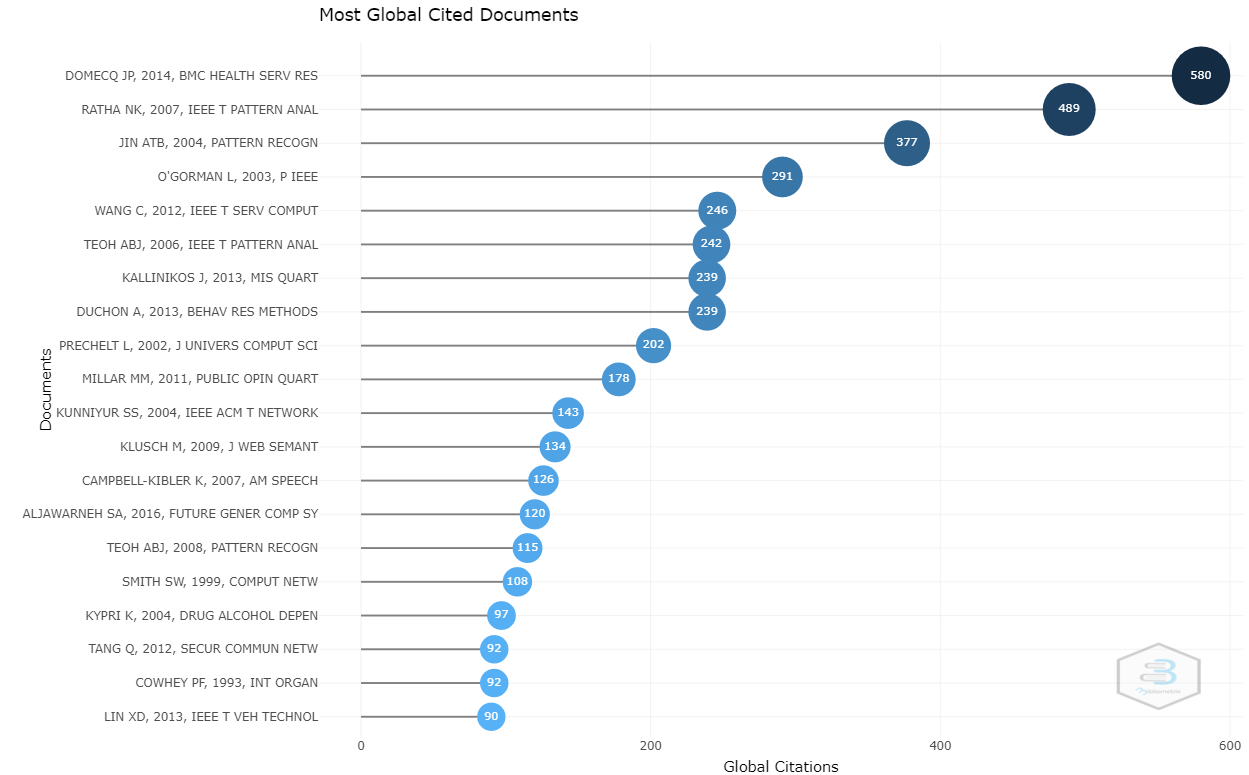
\includegraphics[width=1\textwidth]{experiments/AllannH/PesquisaBibliometrica/Imagens/TSW-AllannH-artigos_citados.png}
    \caption{Os artigos mais citados por outros autores.}
    \label{fig:AllannH-artigos_citados}
\end{figure}

\subsection{Palavras mais utilizadas}
As palavras com o maior numero de ocorrências além das presentes na query de busca mostra o crescimento da segurança em relação a autenticação nos serviços, o crescimento da Blockchain, e com menos da metade de relevância aparece pontos que tendem a crescer como a privacidade e internet of things(IOT).

\begin{figure}
    \centering
    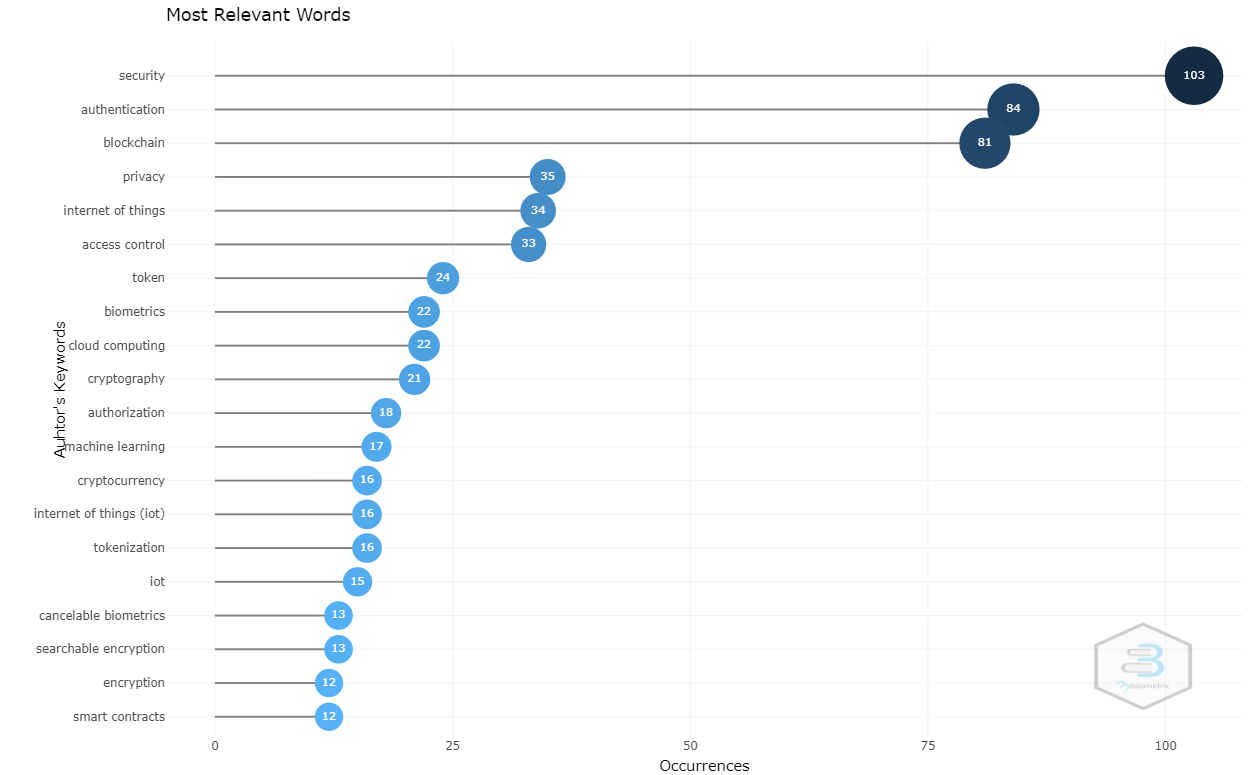
\includegraphics[width=1\textwidth]{experiments/AllannH/PesquisaBibliometrica/Imagens/TSW-AllannH-palavras_relevantes.png}
    \caption{Keywords predominantes na analise.}
    \label{fig:AllannH-palavras_relevantes}
\end{figure}